\documentclass[tikz,border=2pt]{standalone}
\usepackage[T1]{fontenc}
\usepackage[scaled=0.95]{helvet}
\renewcommand{\familydefault}{\sfdefault}
\usetikzlibrary{arrows.meta}
% Volume I chapter dependency map. Palette and flat-block style follow the
% Volume I stack diagrams (ml_systems_stack): muted crimson blocks, white bold type.
% Edges: a later chapter cites an earlier chapter's sections at least twice by
% @sec- reference (python cells excluded), transitively reduced; the introduction
% also points to any chapter with no other incoming edge. Recheck when chapters change.
\definecolor{stackfill}{RGB}{201,119,131}
\definecolor{stackedge}{RGB}{165,28,48}
\definecolor{bandfill}{RGB}{248,236,238}
\definecolor{ink}{RGB}{38,38,42}
\definecolor{softink}{RGB}{105,105,110}
\tikzset{
  band/.style={fill=bandfill,draw=none},
  ptitle/.style={anchor=west,inner sep=0pt,text=ink,font=\bfseries\fontsize{8.2}{9}\selectfont},
  psub/.style={anchor=west,inner sep=0pt,text=softink,font=\fontsize{6.6}{7.8}\selectfont},
  clab/.style={inner sep=0pt,text=white,font=\fontsize{5.6}{6.4}\selectfont},
  ctit/.style={inner sep=0pt,text=white,font=\bfseries\fontsize{7}{8}\selectfont},
  dep/.style={draw=stackedge,line width=0.9pt,-{Stealth[length=4.2pt,width=3.6pt]},rounded corners=0pt}
}
\begin{document}
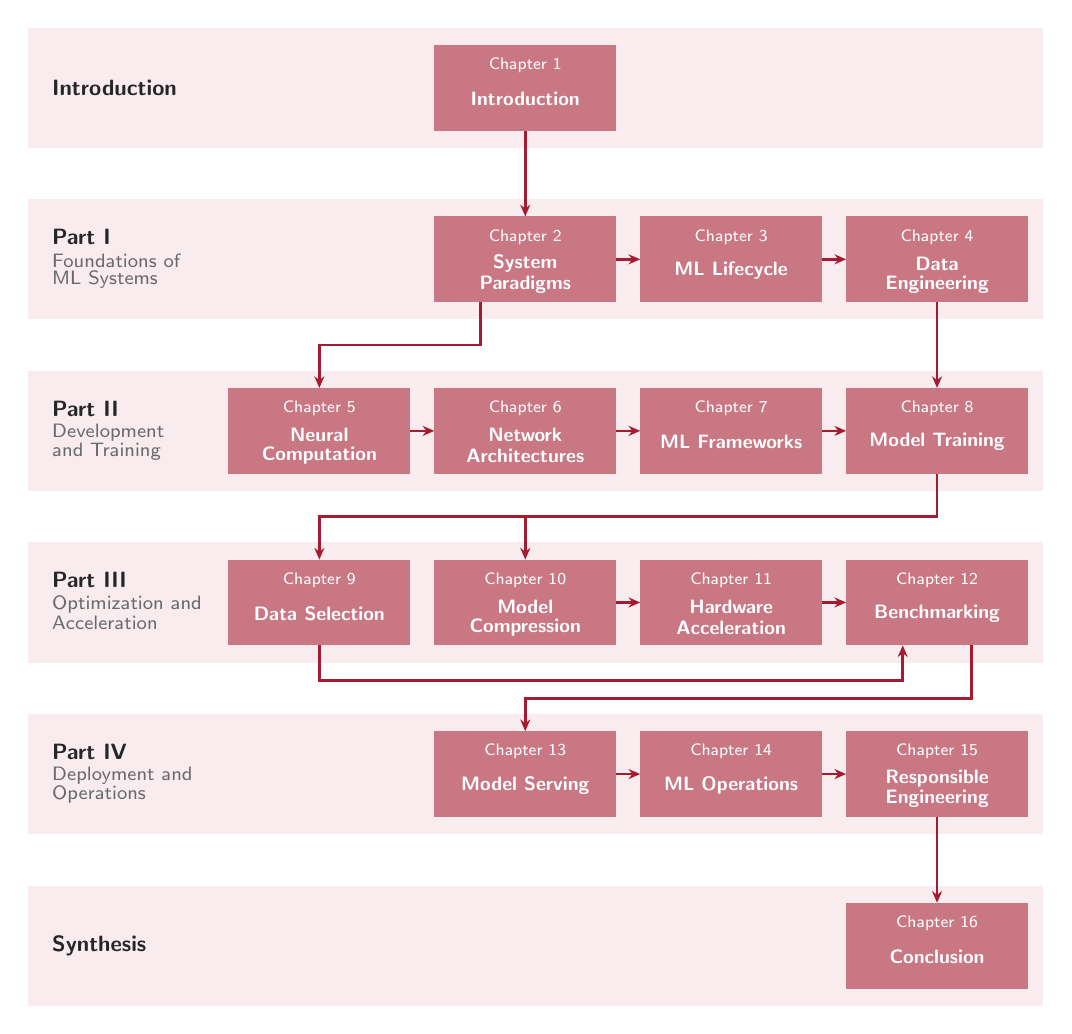
\begin{tikzpicture}[x=1pt,y=-1pt]

\fill[bandfill] (6.20,6.20) rectangle (373.24,49.60);
\node[ptitle] at (14.88,27.90) {Introduction};
\fill[bandfill] (6.20,68.20) rectangle (373.24,111.60);
\node[ptitle] at (14.88,81.84) {Part I};
\node[psub] at (14.88,90.52) {Foundations of};
\node[psub] at (14.88,97.34) {ML Systems};
\fill[bandfill] (6.20,130.20) rectangle (373.24,173.60);
\node[ptitle] at (14.88,143.84) {Part II};
\node[psub] at (14.88,152.52) {Development};
\node[psub] at (14.88,159.34) {and Training};
\fill[bandfill] (6.20,192.20) rectangle (373.24,235.60);
\node[ptitle] at (14.88,205.84) {Part III};
\node[psub] at (14.88,214.52) {Optimization and};
\node[psub] at (14.88,221.34) {Acceleration};
\fill[bandfill] (6.20,254.20) rectangle (373.24,297.60);
\node[ptitle] at (14.88,267.84) {Part IV};
\node[psub] at (14.88,276.52) {Deployment and};
\node[psub] at (14.88,283.34) {Operations};
\fill[bandfill] (6.20,316.20) rectangle (373.24,359.60);
\node[ptitle] at (14.88,337.90) {Synthesis};
\fill[stackfill] (153.14,12.40) rectangle (218.86,43.40);
\node[clab] at (186.00,19.84) {Chapter 1};
\node[ctit] at (186.00,31.93) {Introduction};
\fill[stackfill] (153.14,74.40) rectangle (218.86,105.40);
\node[clab] at (186.00,81.84) {Chapter 2};
\node[ctit] at (186.00,91.45) {System};
\node[ctit] at (186.00,98.89) {Paradigms};
\fill[stackfill] (227.54,74.40) rectangle (293.26,105.40);
\node[clab] at (260.40,81.84) {Chapter 3};
\node[ctit] at (260.40,93.93) {ML Lifecycle};
\fill[stackfill] (301.94,74.40) rectangle (367.66,105.40);
\node[clab] at (334.80,81.84) {Chapter 4};
\node[ctit] at (334.80,91.45) {Data};
\node[ctit] at (334.80,98.89) {Engineering};
\fill[stackfill] (78.74,136.40) rectangle (144.46,167.40);
\node[clab] at (111.60,143.84) {Chapter 5};
\node[ctit] at (111.60,153.45) {Neural};
\node[ctit] at (111.60,160.89) {Computation};
\fill[stackfill] (153.14,136.40) rectangle (218.86,167.40);
\node[clab] at (186.00,143.84) {Chapter 6};
\node[ctit] at (186.00,153.45) {Network};
\node[ctit] at (186.00,160.89) {Architectures};
\fill[stackfill] (227.54,136.40) rectangle (293.26,167.40);
\node[clab] at (260.40,143.84) {Chapter 7};
\node[ctit] at (260.40,155.93) {ML Frameworks};
\fill[stackfill] (301.94,136.40) rectangle (367.66,167.40);
\node[clab] at (334.80,143.84) {Chapter 8};
\node[ctit] at (334.80,155.93) {Model Training};
\fill[stackfill] (78.74,198.40) rectangle (144.46,229.40);
\node[clab] at (111.60,205.84) {Chapter 9};
\node[ctit] at (111.60,217.93) {Data Selection};
\fill[stackfill] (153.14,198.40) rectangle (218.86,229.40);
\node[clab] at (186.00,205.84) {Chapter 10};
\node[ctit] at (186.00,215.45) {Model};
\node[ctit] at (186.00,222.89) {Compression};
\fill[stackfill] (227.54,198.40) rectangle (293.26,229.40);
\node[clab] at (260.40,205.84) {Chapter 11};
\node[ctit] at (260.40,215.45) {Hardware};
\node[ctit] at (260.40,222.89) {Acceleration};
\fill[stackfill] (301.94,198.40) rectangle (367.66,229.40);
\node[clab] at (334.80,205.84) {Chapter 12};
\node[ctit] at (334.80,217.93) {Benchmarking};
\fill[stackfill] (153.14,260.40) rectangle (218.86,291.40);
\node[clab] at (186.00,267.84) {Chapter 13};
\node[ctit] at (186.00,279.93) {Model Serving};
\fill[stackfill] (227.54,260.40) rectangle (293.26,291.40);
\node[clab] at (260.40,267.84) {Chapter 14};
\node[ctit] at (260.40,279.93) {ML Operations};
\fill[stackfill] (301.94,260.40) rectangle (367.66,291.40);
\node[clab] at (334.80,267.84) {Chapter 15};
\node[ctit] at (334.80,277.45) {Responsible};
\node[ctit] at (334.80,284.89) {Engineering};
\fill[stackfill] (301.94,322.40) rectangle (367.66,353.40);
\node[clab] at (334.80,329.84) {Chapter 16};
\node[ctit] at (334.80,341.93) {Conclusion};
\draw[dep] (186.00,43.40) -- (186.00,74.40);
\draw[dep] (218.86,89.90) -- (227.54,89.90);
\draw[dep] (293.26,89.90) -- (301.94,89.90);
\draw[dep] (169.88,105.40) -- (169.88,120.90) -- (111.60,120.90) -- (111.60,136.40);
\draw[dep] (334.80,105.40) -- (334.80,136.40);
\draw[dep] (144.46,151.90) -- (153.14,151.90);
\draw[dep] (218.86,151.90) -- (227.54,151.90);
\draw[dep] (293.26,151.90) -- (301.94,151.90);
\draw[dep] (334.80,167.40) -- (334.80,182.90) -- (111.60,182.90) -- (111.60,198.40);
\draw[dep] (334.80,167.40) -- (334.80,182.90) -- (186.00,182.90) -- (186.00,198.40);
\draw[dep] (218.86,213.90) -- (227.54,213.90);
\draw[dep] (293.26,213.90) -- (301.94,213.90);
\draw[dep] (111.60,229.40) -- (111.60,242.11) -- (322.40,242.11) -- (322.40,229.40);
\draw[dep] (347.20,229.40) -- (347.20,248.62) -- (186.00,248.62) -- (186.00,260.40);
\draw[dep] (218.86,275.90) -- (227.54,275.90);
\draw[dep] (293.26,275.90) -- (301.94,275.90);
\draw[dep] (334.80,291.40) -- (334.80,322.40);
\end{tikzpicture}
\end{document}
